\chapter{System Design}
\setcounter{equation}{0}

\section{Architecture}
The architecture follows four layers. The extension layer observes browser events and
provides immediate warnings or supported restrictions. The processing layer contains
the FastAPI service and detector orchestration. The intelligence layer contains
XGBoost, Random Forest, static-analysis rules, threat-intelligence integrations, and
the RAG/LLM workflow. The dashboard and persistence layer provides authenticated
interaction, reports, analytics, and Firebase identity.

\section{Use Case Diagram}
The primary use cases are monitoring browsing activity, scanning a URL or QR code,
inspecting a webpage, analyzing a download or email, reviewing evidence, receiving a
warning, and viewing authorized history. The user can request a deeper dashboard
analysis, while the system administrator manages configuration and authorized analysts
review reports.
\begin{figure}[H]
    \centering
    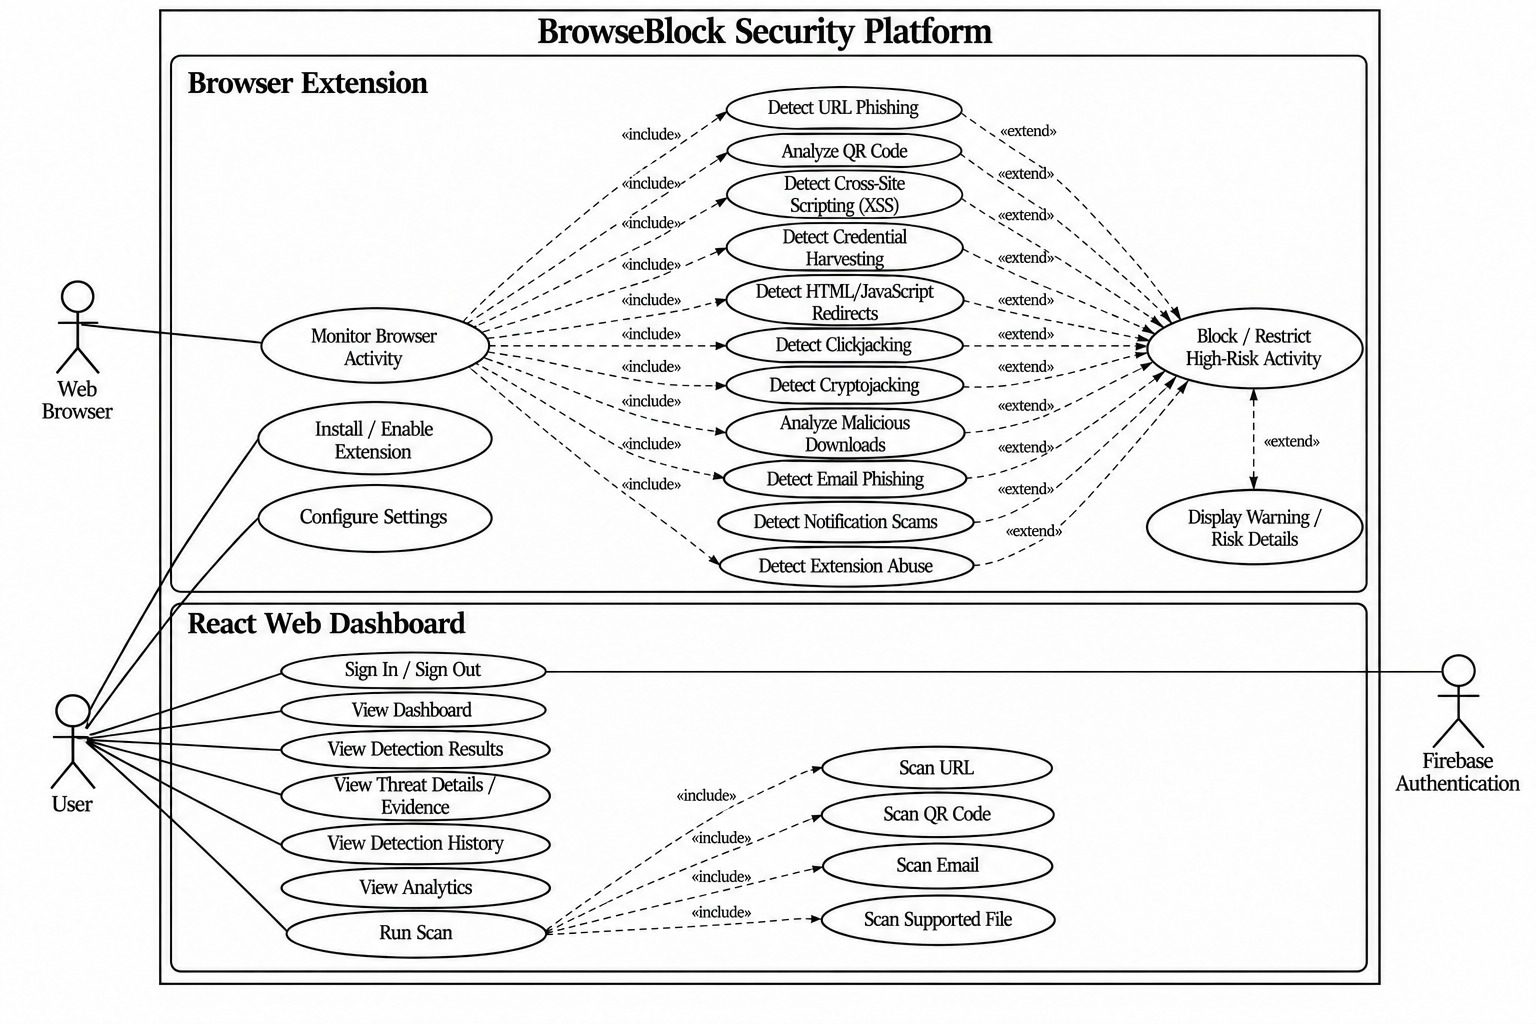
\includegraphics[width=\textwidth]{images/useCase.png}
    \caption{BrowseBlock use case diagram}
\end{figure}

\section{Activity Diagram}
The BrowseBlock workflow begins with a browser event or manual scan. The system
validates the input, selects the relevant detector, extracts observable evidence, and
performs model and rule-based analysis. It then assigns a risk level, explains the
indicators, applies a warning or protective action where supported, and records the
result according to privacy and retention policy. Unsupported input, timeout, or
incomplete evidence produces an explicit limitation rather than a safe result.
\begin{figure}[H]
    \centering
    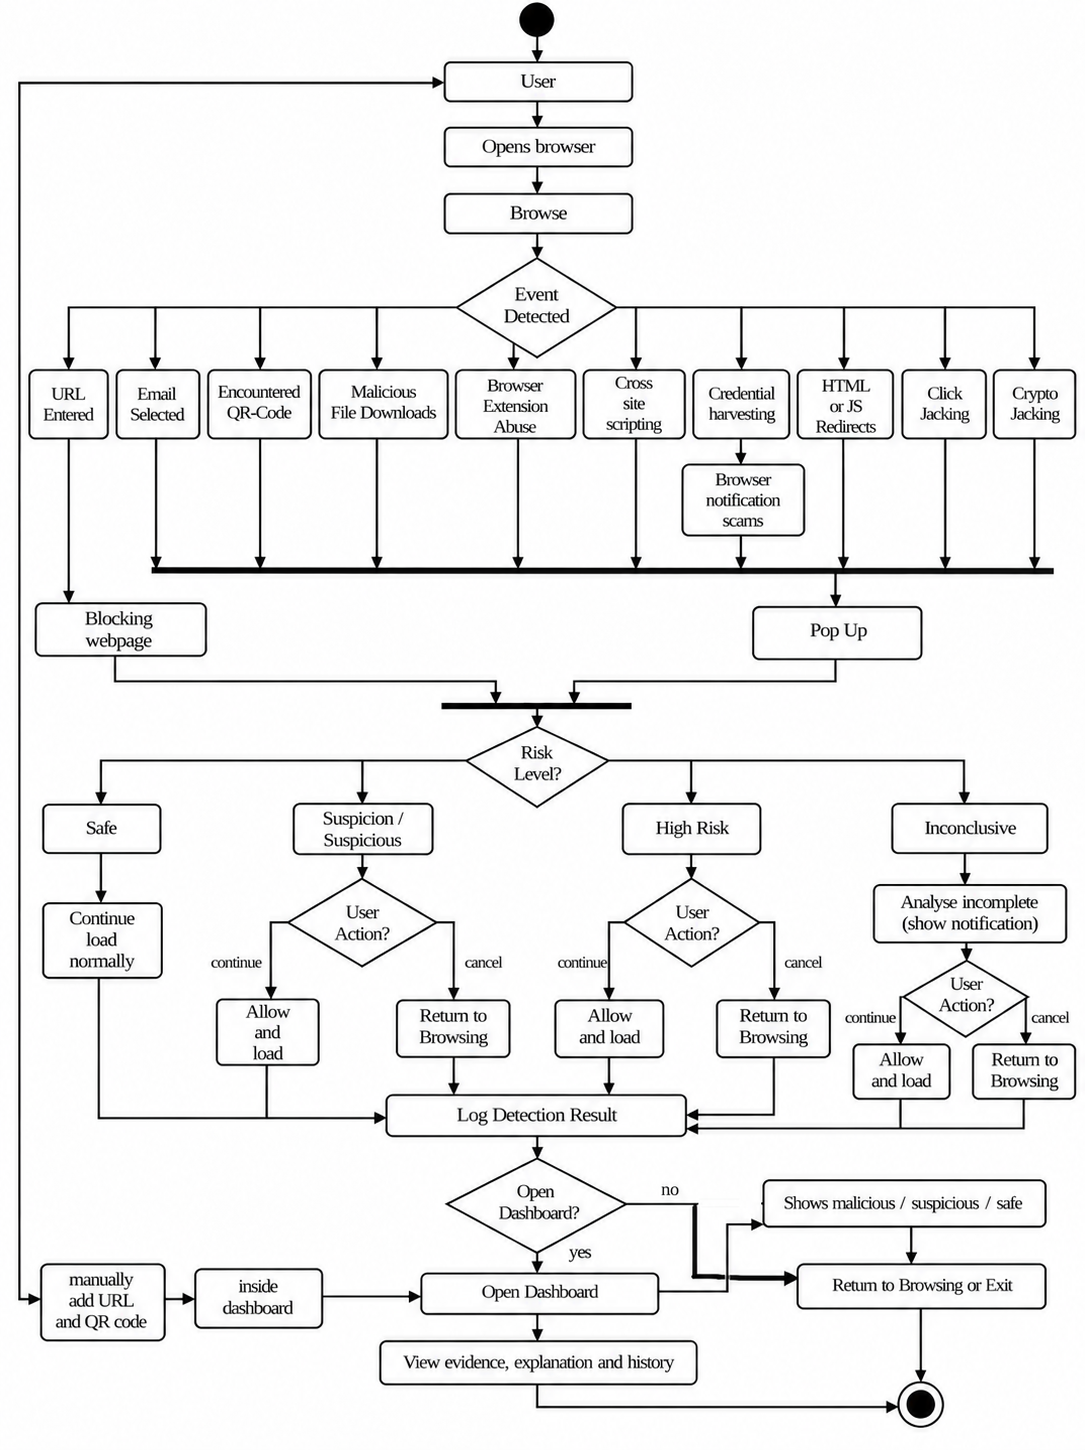
\includegraphics[width=0.6\textwidth,height=0.55\textheight,keepaspectratio]{images/ActivityDiagram.png}
    \caption{BrowseBlock activity diagram}
\end{figure}

\newpage
\section{Sequence Diagram}
For a navigation event, the extension captures the URL and available context, sends
only the required request to the backend, and receives a risk assessment and evidence.
The extension displays the result and applies a supported rule when appropriate. For a
dashboard scan, Firebase authenticates the user, FastAPI verifies the ID token,
coordinates the selected detector and returns the authorized result, and
returns a report. At every stage, failed analysis and unavailable enforcement are
reported explicitly.
\IfFileExists{images/architecture.png}{%
    \begin{figure}[H]
        \centering
        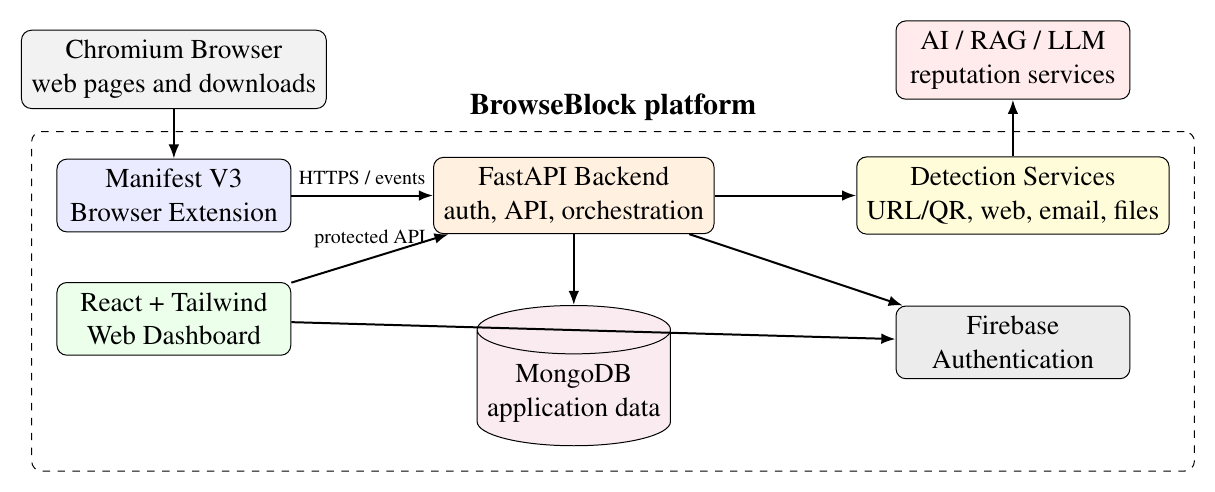
\includegraphics[width=\textwidth]{images/architecture.png}
        \caption{BrowseBlock architecture}
    \end{figure}
}{%
    \PackageWarning{chapter5}{Missing images/architecture.png; architecture diagram omitted}%
}

\section{Data Model}
The data model associates authenticated users with scan requests, detection results,
threat reports, and audit records. A result stores the detector category, risk level,
indicators, timestamp, analysis completeness, and protective action. File hashes and
minimal metadata may be retained according to policy; raw email, webpage, URL
parameters, and file contents are not retained unnecessarily.
\begin{figure}[H]
    \centering
    \makebox[\textwidth][l]{%
        \hspace*{-2.5cm}%
        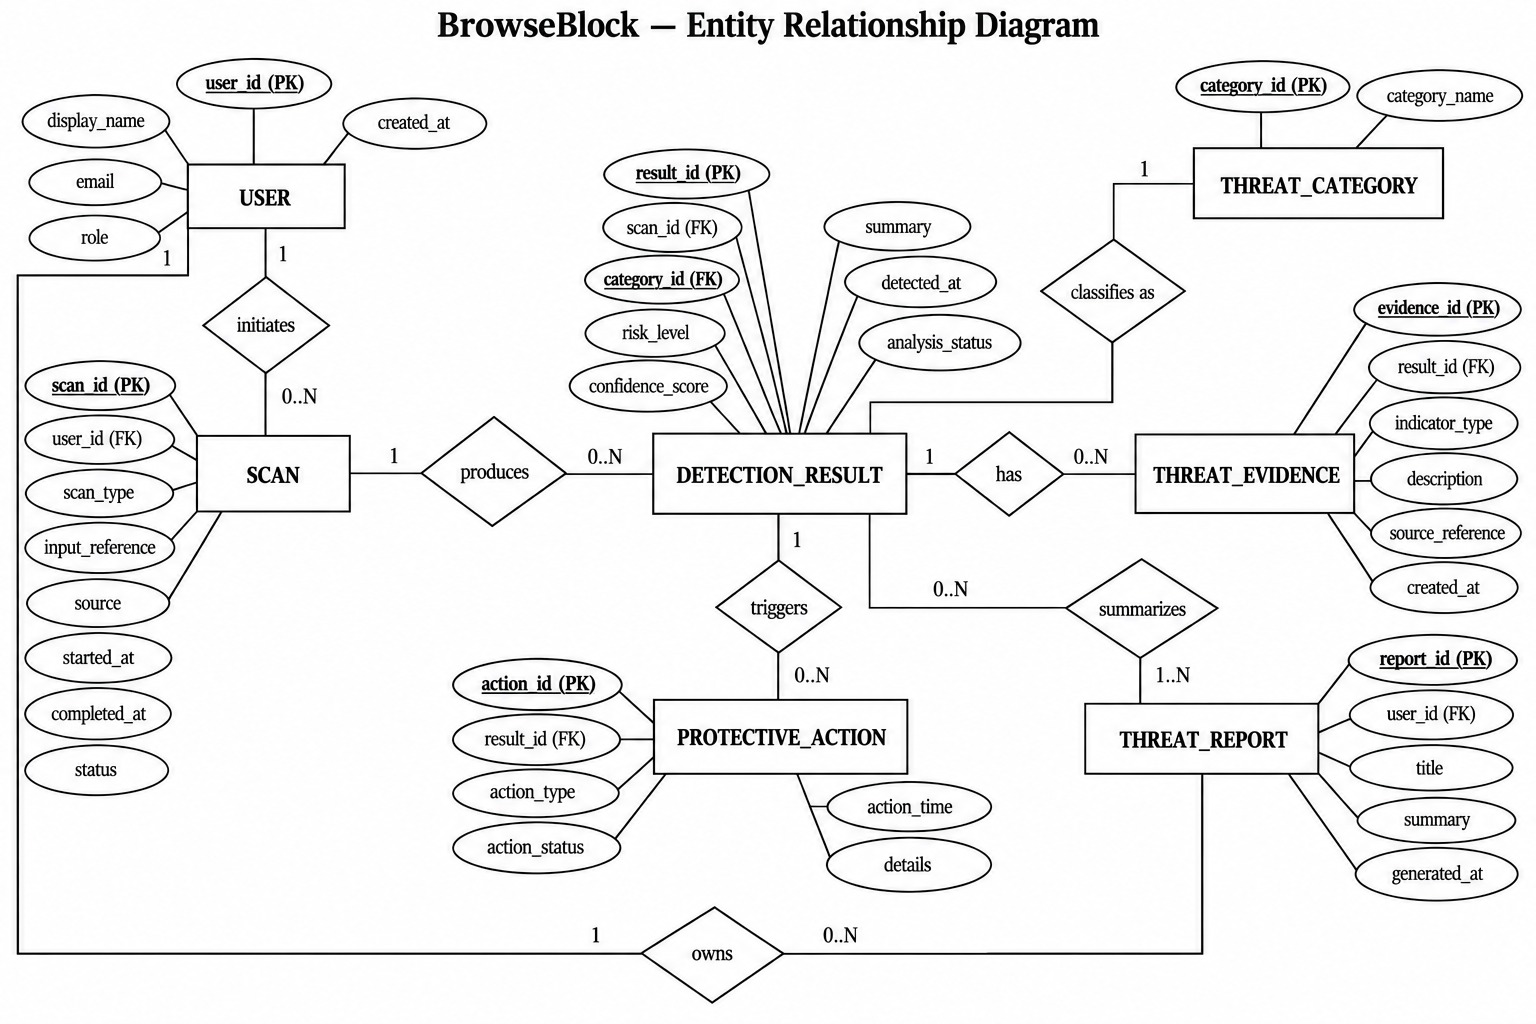
\includegraphics[width=0.98\paperwidth,height=0.98\textheight,keepaspectratio]{images/ERdiagram.png}%
    }
    \caption{BrowseBlock entity relationship diagram}
\end{figure}
